%(BEGIN_QUESTION)
% Copyright 2006, Tony R. Kuphaldt, released under the Creative Commons Attribution License (v 1.0)
% This means you may do almost anything with this work of mine, so long as you give me proper credit

Regn ut trykket på utløpet av dette røret ($P_2$), dersom vi antar at det strømmer vann ($\rho = 998.19$) og at strømningen skjer uten friksjon (altså uten trykktap mot rørveggen).

$$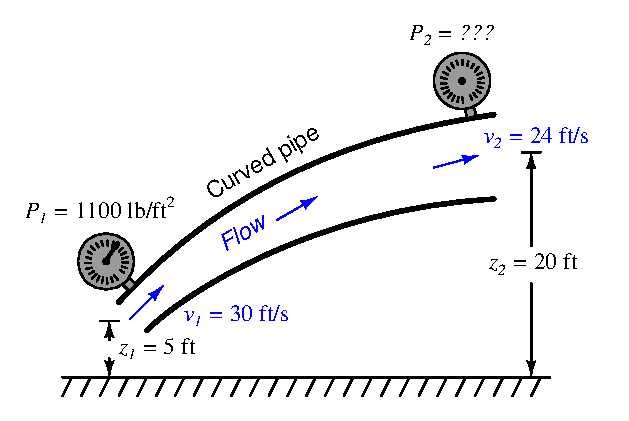
\includegraphics[width=15.5cm]{i00450x01.eps}$$

\vskip 10pt

\noindent
{\bf Bernoullis ligning:}

$$z_1 \rho g + {v_1^2 \rho \over 2} + P_1 = z_2 \rho g + {v_2^2 \rho \over 2} + P_2$$

\vskip 20pt \vbox{\hrule \hbox{\strut \vrule{} {\bf Forslag til sokratisk diskusjon} \vrule} \hrule}

\begin{itemize}
\item{} En vanlig feil når elever løser oppgaver med Bernoullis lov, er å bruke enheter som ikke passer sammen. Vis hvordan alle oppgitte måleenheter i denne oppgaven faktisk er kompatible i formen de er gitt, uten behov for enhetskonvertering.
\end{itemize}

\underbar{file i00450}
%(END_QUESTION)





%(BEGIN_ANSWER)

$P_2$ = 31.39 kPa

\vskip 10pt

Det kan være fristende å endre Bernoullis ligning slik at målinger i tommer kan brukes i stedet for fot (særlig den «plagsomme» trykkenheten pund per kvadrat{\it fot}, i stedet for PSI). Man må likevel være forsiktig, fordi det er mer enn bare å bytte ut «ft» med «in» i ligningen.

$$z_1 \rho g + {v_1^2 \rho \over 2} + P_1 = z_2 \rho g + {v_2^2 \rho \over 2} + P_2$$

Enheten «fot» ligger også skjult inne i enheten «slug», og dette må tas hensyn til. Her er standard sammenheng mellom vekt, masse og tyngdeakselerasjon:

$$W = mg$$

$$[\hbox{lb}] = [\hbox{slug}] \left[ \hbox{ft} \over \hbox{s}^2 \right]$$

Hvis vi skriver enhetsanalysen slik at slug vises som sammensatt enhet, ser vi at «fot» inngår:

$$[\hbox{lb}] = \left[{\hbox{lb} \cdot \hbox{s}^2} \over \hbox{ft}\right] \left[ \hbox{ft} \over \hbox{s}^2 \right]$$

Dermed vil det å uttrykke $g$ i tommer per sekund i andre kreve at vi innfører en ny masseenhet (lb $\cdot$ s$^{2}$ per in) i stedet for slug (lb $\cdot$ s$^{2}$ per ft).

%(END_ANSWER)





%(BEGIN_NOTES)


%INDEX% Physics, dynamic fluids: Bernoulli's equation

%(END_NOTES)
